\section{Изучение вибраторных антенн}

\subsection{Симметричный вибратор}

В простейшем случае состоит из двух токопроводящих отрезков, каждый из которых равен $1/4$ длины волны. В симметричном вибраторе провода линии — вибраторы разведены на $180^{\circ}$.

\begin{figure}[H]
    \centering
    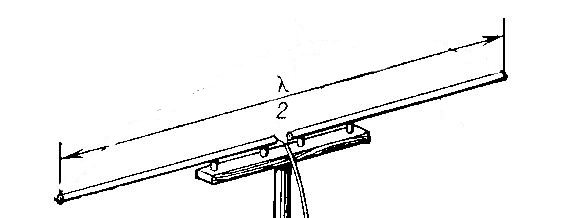
\includegraphics[width=.9\textwidth]{img/1.jpg}
    \caption{Симметричный вибратор}
\end{figure}

Широко применяется для приема телевизионных передач, как самостоятельно, так и в составе комбинированных антенн.
Так, к примеру, если диапазон метровых волн телепередач проходит через отметку $200$ МГц, то длина волны будет равна $1.5$ м.
Каждый отрезок симметричного вибратора будет равен $0.375$ метра.

\begin{figure}[H]
    \centering
    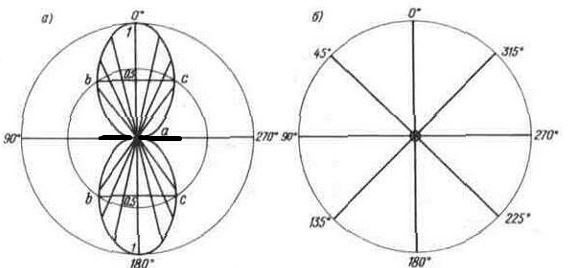
\includegraphics{img/2.jpg}
    \caption{Диаграмма направленности симметричного вибратора}
\end{figure}


\subsection{Несимметричный вибратор}

Или попросту штыревая антенна, представляет из себя <<половину>> симметричного вибратора, установленного вертикально.
В качестве длины вибратора, применяют $1$, $1/2$ или $1/4$ длины волны.

\begin{figure}[H]
    \centering
    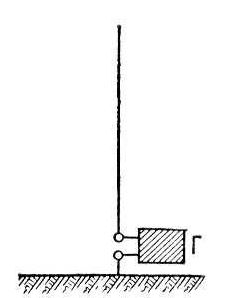
\includegraphics{img/3.jpg}
    \caption{Несимметричный вибратор}
\end{figure}


\begin{figure}[H]
    \centering
    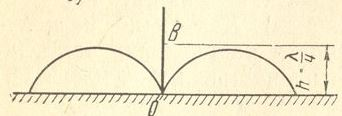
\includegraphics{img/4.jpg}
    \caption{Диаграмма направленности несимметричного вибратора}
\end{figure}

Представляет собой рассеченную вдоль <<восьмерку>>. За счет того, что вторая половина <<восьмерки>> поглощается землей, коэффициент направленного действия у несимметричного вибратора в два раза больше, чем у симметричного, за счет того, что вся мощность излучается в более узком направлении.
Основное применение, в диапазонах ДВ, КВ, СВ, активно устанавливаются в качестве антенн на транспорте.

\subsection{Петлевой вибратор}

Два одинаковых вибратора могут быть размещены на небольшом расстоянии, параллельно друг другу. Если при этом соединить между собой концы этих вибраторов, а нижний вибратор разрезать посередине получится так называемый петлевой вибратор. Практически простой полуволновый вибратор и петлевой полуволновый вибратор имеют похожие рабочие характеристики.

\begin{figure}[H]
    \centering
    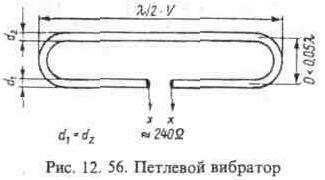
\includegraphics{img/petl.jpg}
    \caption{Петлевой вибратор}
\end{figure}

Петлевой вибратор выполняют из тех же материалов, что и разрезной. Радиус закругления концов петлевого вибратора не имеет значения. В точках питания концы трубок можно расплющить. Коэффициент укорочения полуволнового петлевого вибратора значительно меньше зависит от диаметра трубки, чем коэффициент укорочения разрезного вибратора. Поэтому длина петлевого вибратора, выполненного из трубок диаметром $10 ... 20$ мм, практически остается неизменной. Механическое соединение петлевого вибратора с мачтой можно выполнять любым способом: сваркой, заклепочным или винтовым соединением без изоляции.


\subsection{Волновой канал}

Антенны типа <<Волновой канал>> получили широкое распространение в различных профессиональных устройствах радиосвязи и радиолокации. Большинство телевизионных коллективных и индивидуальных антенн промышленного изготовления также являются антеннами типа <<Волновой канал>>. Это связано с тем, что такие антенны достаточно компактны и обеспечивают получение большого коэффициента усиления при сравнительно небольших габаритах. Иногда антенну <<Волновой канал>>, особенно в зарубежной литературе, называют антенной Уда-Яги по имени впервые описавших ее японских изобретателей.

Антенна <<Волновой канал>> представляет собой набор элементов: активного - вибратора и пассивных - рефлектора и нескольких директоров, установленных на одной общей стреле.

\begin{figure}[H]
    \centering
    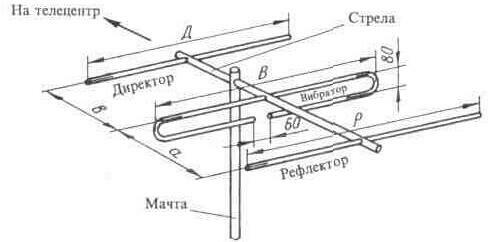
\includegraphics[width=.9\textwidth]{img/uda-yagi.jpg}
    \caption{Трехэлементная антенна <<Волновой канал>>}
\end{figure}

Принцип действия антенны в следующем. Вибратор определенной длины, находящийся в электромагнитном поле сигнала, резонирует на частоте сигнала, и в нем наводится ЭДС. В каждом из пассивных элементов также наводится ЭДС, и они переизлучают вторичные электромагнитные поля. Эти вторичные поля, в свою очередь, наводят дополнительные ЭДС в вибраторе. Размеры пассивных элементов и их расстояния от вибратора должны быть выбраны такими, чтобы дополнительные ЭДС, наведенные в вибраторе вторичными полями, были в фазе с основной ЭДС, наведенной в нем первичным полем. Тогда все ЭДС будут складываться арифметически, обеспечив увеличение эффективности антенны по сравнению с одиночным вибратором. Для этого рефлектор делается немного длиннее вибратора, а директоры - короче.